
\title{

\twoauthors
  {Jamie Bullock} {UCE Birmingham Conservatoire \\ Music Technology}
  {Henrik Frisk} {Lund University\\
    Malm\"{o} Academy of Music\\ 
    Composition and Performance}

\begin{document}
%
\maketitle
%
\begin{abstract}
In this paper we describe a means of storing information about audio and message processing modules, which is not software specific. This information includes a module description, module instance data, and module implementation data. A novel XML file format and database schema are proposed, and we show how a newly developed library (libIntegra) can be used as a link between persistent storage on a networked server, and an existing software environment for audio. The library provides methods for instantiating and connecting modules in a given piece of software, and addressing them using Open Sound Control (OSC) messaging. 
\end{abstract}

\section{The Integra project}\label{sec:integra_introduction}

libIntegra is part of the Integra project, a 3-year project led by UCE Birmingham Conservatoire in the UK and part financed by Culture 2000\footnote{\url{http://www.integralive.org}}. The Integra library is being developed as a foundation for the software development aspect of the project. 

\section{Integra modules}\label{sec:modules}

The basis of the Integra library is the concept of the Integra module. Integra modules encapsulate a specific piece of message or signal processing functionality. A module could perform a simple task like a numeric addition, or a complex task like emulating a specific synthesiser. In this section, we will outline how Integra modules and module collections are constructed.

\subsection{Module construction}\label{subsec:module_construction}

The minimum requirement for an Integra module is that it must have an interface definition. In addition, it may also have an implementation and module instance data. Of these, only the implementation is software specific.

\subsubsection{Module definition}\label{subsubsec:module_definition}

An Integra module definition is data that defines what attributes a
module has, and what the characteristics of those attributes are. An
Integra attribute is a symbolic name with which a value can be
associated. The module definition does not store the actual values of
attributes, instead it stores data about the attributes such as their
names, descriptions, supported data types, maxima and minima, and
default values. Typical module definition data is shown in Table
\ref{tab:module_definition}.

\begin{table}
\begin{center}
\begin{tabular}{|l|l|}
\hline
\textbf{Field} & \textbf{Value} \\
\hline
Name  & Oscillator \\
\hline
Parent  & Module \\
\hline
Attributes & freq, phase \\
\hline
Attribute Unit Codes & 1, 2 \\
\hline
Attribute Minima & 0, 0 \\
\hline
Attribute Maxima & inf, 6.2831853071795862 \\
\hline
Attribute Defaults & 440, 0 \\
\hline
\end{tabular} 
\end{center}
\caption{Integra Oscillator interface definition}
\label{tab:module_definition}
\end{table}

The parent field is used to show an inheritance relation. All Integra module definitions could be thought of as class definitions, the members of which are all abstract (lack implementation), or interface definitions. The interface of a given class can inherit the interface of any other class, and supplement this with additional members. This definition hierarchy is the basis of the Integra database (see section \ref{subsec:serialization}). 

\subsubsection{Module namespace}\label{subsubsec:module_namespace}

A module's namespace is derived from its definition. The namespace
enables the values of attributes to be set, and module methods to be
called by using a symbolic naming scheme.  From the user's
perspective, this will usually manifest itself as an automatically
generated OSC address space. The OSC address space for a Sinus module
is shown in table \ref{tab:module_namespace}. The 'Sinus' class
inherits the 'Oscillator' class interface, which in turn inherits the
'Module' class interface, so the attributes of these inherited classes
must be reflected in the Sinus module's namespace. To keep addresses
short, class names are omitted from the namespace unless there is a
name clash.

\begin{table}
\begin{center}
\begin{tabular}{|p{13em}|p{8em}|}
\hline
\textbf{OSC address} & \textbf{Purpose} \\
\hline
\begin{minipage}[0pt]{10em}
\footnotesize {
\begin{verbatim}/<modulename>/freq <value>\end{verbatim}}\end{minipage}  & \small{Set the value of the 'freq' attribute} \\
\hline
\begin{minipage}[0pt]{10em}
\footnotesize {
\begin{verbatim}/<modulename>/phase <value>\end{verbatim}}\end{minipage}  & \small{Set the value of the 'phase' attribute} \\
\hline
\begin{minipage}[0pt]{10em}
\footnotesize {
\begin{verbatim}/<modulename>/active <value>
\end{verbatim}} \end{minipage} & \small{Set whether or not the module is active} \\
\hline
\end{tabular} 
\end{center}
\caption{Integra Sinus module namespace}
\label{tab:module_namespace}
\end{table}

\subsubsection{Module implementation}\label{subsubsec:module_implementation}

The module implementation is the only software-specific data stored by Integra. It consists of a fragment of computer code, in one or more files, which when run or loaded by a particular piece of software will perform a specific audio or message processing task. In order that module implementations can be used by libIntegra, an implementation protocol must be devised for each software target. This protocol must then supported by the target-specific libIntegra bridge (see figure \ref{fig:model}).

Integra currently provides implementation protocols for Max/MSP and Pure Data along with a growing selection of example module implementations and implementation templates. An eventual aim of Integra is to provide a protocol for constructing module implementations in a range of different software, and to develop a LADSPA/DSSI\footnote{\url{http://dssi.sourceforge.net/}} host that wraps plugins in an Integra-compliant manner.

\subsubsection{Module instance data}\label{subsubsec:module_instance_data} 

Module instance data consists of the run-time state of all of its variable parameters. This data is stored in memory by the Integra library whilst a module is in use, and can be written to an XML file on demand. This data is stored in the Integra database in the module's instance table. However only one saved state can be associated with each module instance. If the user wishes to record state changes over time, then a separate 'Player' module must be used to store this data.

\subsection{Module collections}\label{subsec:module_collections}

An Integra collection consists of one or more Integra module instances. A collection can also contain other collections. These contained collections encapsulate the functionality of a number of connected Integra modules into a single entity and can be addressed and connected as if they were normal module instances. The facility is provided for collections to optionally expose the input and output parameters of the modules they contain. For example, the collection 'mySinus' might contain a Sinus module, which has the attributes Frequency and Phase, but the collection might only expose the Frequency attribute to the containing collection, whilst setting the Phase to some arbitrary constant value.

\subsection{Module ports}\label{subsec:module_ports} 

Modules and collections are connected up to each other using Integra ports. Each port corresponds to an audio or messaging address, which has both a symbolic name and a numeric identifier (port ID). Port symbolic names correspond to a module's attribute names (e.g. 'freq'), and port numbers are derived implicitly from the index of the port in the module's attribute list. In addition to its port numbers, each module has a globally unique symbolic name (e.g. 'sinus1'), and an implicitly determined, globally unique numeric identifier (UID). The Integra library can be used to address any module port using either its symbolic name and attribute name (e.g. '/sinus1/freq'), or using a combination of its UID and port ID. It is an important part of the Integra module construction protocol that port ordering is always consistent. Otherwise a module implementation's port numbering will not correspond to the numbering expected by the Integra library.

From the perspective of the Integra library, database, and XML schema,
there is no distinction between audio and control rate ports. This
distinction is only made in the implementation. There is also no
conceptual distinction between input ports and output ports; a port is
just an address that can receive data and connect to other addresses.

\subsection{Connections}\label{subsec:connections}

For each module or collection, the Integra library stores a list of ports that each output port of a given module is connected to. One-to-many, many-to-one or many-to-many connections can easily be established. It is important to note that for audio connections, the software hosting the modules must support the required routings. This is because the library doesn't currently process audio-rate data.

\section{IXD (Integra eXtensible Data)}\label{sec:ixd}

In order to store modules, module collections, and performance data in a software-neutral manner, a bespoke Integra file format was developed. XML was chosen as the basis for this since it is relatively human-readable, can be transformed for a variety of output targets, and has a number of excellent tools for parsing, reading and writing. 

Rather than keeping all data needed to store an Integra collection in a single file we make use of the XML Linking language (XLink\footnote{\url{http://www.w3.org/TR/xlink/}}) to link in relevant resources. This makes for more efficient parsing and helps to keep file sizes small.

\subsection{Integra module definition}\label{subsect:integra_class_definition}

Perhaps the most important part of the IXD specification is the module definition file. It is the XML representation of an Integra module (see \ref{subsubsec:module_definition}). These files are created and updated through the database interface and stored locally for offline access in a gzipped archive. Each file contains the class and module definitions of one unique module and a link to the parent class from which it inherits properties:

{\small
\begin{verbatim}
<Class>
 <ClassDefinition>
   <className>Sinus</className>
   <classParent ...
        xlink:href="Oscillator.xml">
        Oscillator
   </classParent>
    ...
 </ClassDefinition>
 <ModuleDefinition>
    ...
 </ModuleDefinition>
</Class
\end{verbatim}
}
All documents that are part of the Integra documentation system must have a class definition - it represents the super class of the Integra class hierarchy and it defines those attributes shared by all kinds of data - performance data, biographical data, etc. The module definition is specific to the notion of \emph{modules} as defined in section \ref{sec:modules}.

Each module and each of its attributes may also hold a documentation
reference. This allows the implementing host for this module to make a
call to the instance host to bring up on-line documentation, for a
specific attribute or for the module itself. The link points to a file
included in the local archive of module descriptions.

\subsection{Integra collection definition}\label{subsect:integra_collection_definition}

Once a module is defined and stored in an IXD file it may be instantiated. Instances of classes of modules along with their inter-connections are stored in a collection file which is the Integra equivalent of a PD or Max/MSP 'patch'.

In a collection file each module instance is represented by a locator that points to the definition of the class to which the instance belongs. Connections between ports are represented by \emph{arcs} between resources (pointing to definitions of individual addresses) in the module definition file pointed to by the locator. Finally, it also holds references to performance data files.


% \subsection{The IXD file format - summary}
\subsection{Serialization layer}\label{sec:serialization_layer}

To facilitate the conversion between flat XML files conforming to the IXD specification, and a memory-resident representation of the data, a serialization library component has been developed (see \ref{subsec:serialization}). The serialization layer is the link  between the database and the local file system (see figure \ref{fig:model}).

The serialization component provides functions for loading, saving and modifying XML, and is used by the instance host (see \ref{subsec:instance_host}), the database (see \ref{subsec:serialization}) and/or any other application interfacing with the library. For example, on the database server, the serialization layer is made available to the python-based web interface via a SWIG-generated interface.

The IXD format is specified and documented in several XML Schemas\footnote{\url{http://www.w3.org/XML/Schema}}. The XML Schema for the module definition files is closely correlated to the database schema and they share the same versioning system. Any file conforming to the file format can be validated against a specific schema version and conditional actions may be performed on them as appropriate.

Finally, we are also working on an Integra specific XSL Transformation\footnote{\url{http://www.w3.org/TR/xslt}} specification for automatic generation of XHTML and/or PDF documentation of a given module or collection of modules. In practice this means that once the user has created his or her own Integra collection for a project and uploaded it to the database, a documentation file for this collection is automatically generated.


\section{(Integra)tion via the library}\label{subsec:db_lib}

libIntegra is a cross-platform shared library, mostly written in ISO C89 compliant C, and packaged using the GNU autotools tool chain. It consists of a common API, and a number of optional components. The library is hosted on Sourceforge.net\footnote{\url{http://www.sourceforge.net/projects/integralive}} where source code and API documentation can be accessed.

\subsection{Data persistence}\label{subsec:serialization}

For persistent storage of module data and other data relating to musical works we have designed and configured an on-line database. The only way in which users may add new, or edit existing module definitions is via a web-based interface to this database. The database makes use of the libIntegra serialization component to generate XML files on-the-fly, and these files are bundled into a gzipped archive to be downloaded and stored locally for potential offline use. Any program linked to libIntegra can then use the same XML handling functions to de-serialise the data, and form an in-memory representation of it.

\subsection{Instance host}\label{subsec:instance_host}

As well as a serialization component the library provides an instance
host, which is responsible for keeping a record of each module's
run-time state. This includes the values that any of its ports have,
and any connections that are made between modules. The instance host
acts as an OSC server (using the liblo
library\footnote{\url{http://liblo.sourceforge.net/}}), and operations
can be performed on modules by sending OSC messages to it. The
instance host supports a condensed OSC syntax for loading, removing,
connecting, disconnecting and addressing modules. For example two
module ports can be connected with the following message: 
\begin{verbatim}
/connect <module id> <port id> 
         <module id> <port id>
\end{verbatim}

Module instances can either communicate with each other through the instance host using OSC, or using an environment-specific messaging system. When messages pass through the Instance host, various operations can be performed on the data that passes through. These operations include type checking, range checking, unit conversion and type conversion. All of these can be validated against the module definition held in memory.
 
\subsection{Library/target bridge}\label{subsec:bridge}

In order to instantiate modules in a target environment and to communicate directly with these modules, a target-specific 'bridge' is required. The 'bridge' is a dynamically loaded, binary shared object hosted 'inside' the instance host. Its purpose is to facilitate bi-directional communication between the instance host and a given target module host (see \ref{subsec:module_host}). The library provides a very simple API that each target-specific bridge must conform to. The instance host has no knowledge of the software being used to host module instances so the bridge acts like a translator receiving function calls, and performing the relevant target-specific actions. These actions include instantiating modules, removing them and connecting them. Most OSC commands supported by the Instance host have a corresponding function in the bridge.

It is the bridge's software-specific communication mechanism that determines the protocol used to construct module implementations. It is possible, although not necessarily desirable to have several bridges for a given target, each of which elicits a different approach to module construction. This might be useful for compatibility with existing modularisation efforts, such as the Jamoma project or Faust's auto-generated PD abstractions.

\begin{figure}
\centerline{\framebox{
\includegraphics[width=\columnwidth]{img/library_model_small}}}
\caption{A model of the parts constituting libIntegra and how the library interfaces with other parts of the system.}
\label{fig:model}
\end{figure}

\subsection{Module host}\label{subsec:module_host}

The module host is any software that hosts Integra modules: it is not part of libIntegra. Typically, a module host will be dynamically linked to libIntegra at compile time. At run time the module host can make direct calls to functions in the instance host and also make use of the Instance host OSC interface. Typically the OSC interface is used for communication with modules or hosts that are running in a different program or operating system process. Communication from the Instance host to the module host and modules is always achieved through the 'bridge'.

It is also possible for the module host to be a standalone application that doesn't link to libIntegra. In this case the bridge will usually use a network-based protocol such as OSC to communicate with the module host. A Unix pipe or socket is another possibility for this type of setup.

\subsection{Inter-library communication}\label{subsec:interlib}

An arbitrary number of libIntegra instances may be running on the same computer or on any number of networked computers. Each libIntegra instance can be running in a new instance of a common module host, or a completely different module host. A single computer
setup is shown in Figure \ref{fig:model}. 

When multiple libIntegra instances are used, only one (the master), can make use of the serialization layer to load and save Integra module instance data and collections. This is to prevent several versions of the same collection being opened by different library instances, and becoming unsynchronised. If the user or developer knows that the serialization layer will not be required, the library can be compiled without it.

The Instance host contains mechanisms for inter-library communication and auto-discovery. This is mostly achieved through OSC messaging, and facilitates the loading of Integra collections across several module hosts, with transparent state saving.


\section{Conclusion}\label{sec:conclusion}

We have outlined a robust, cross-platform, software-in\-dependent means of storing and loading module data. In addition we have discussed the facilities that the Integra library provides for loading, saving, instantiating and managing modules and collections of modules. The next stage in our work will entail a phase of alpha and beta testing, both internally and with our end-users. The aim of the Integra project is to improve the usability of software for working with live electronics, and to provide a mechanism for the sustainability of the musical works it is used to create. libIntegra should ultimately provide a foundation for this.

\end{document}
